\section{Introduction}
\label{sec:intro}

\begin{figure}[t]
\centering
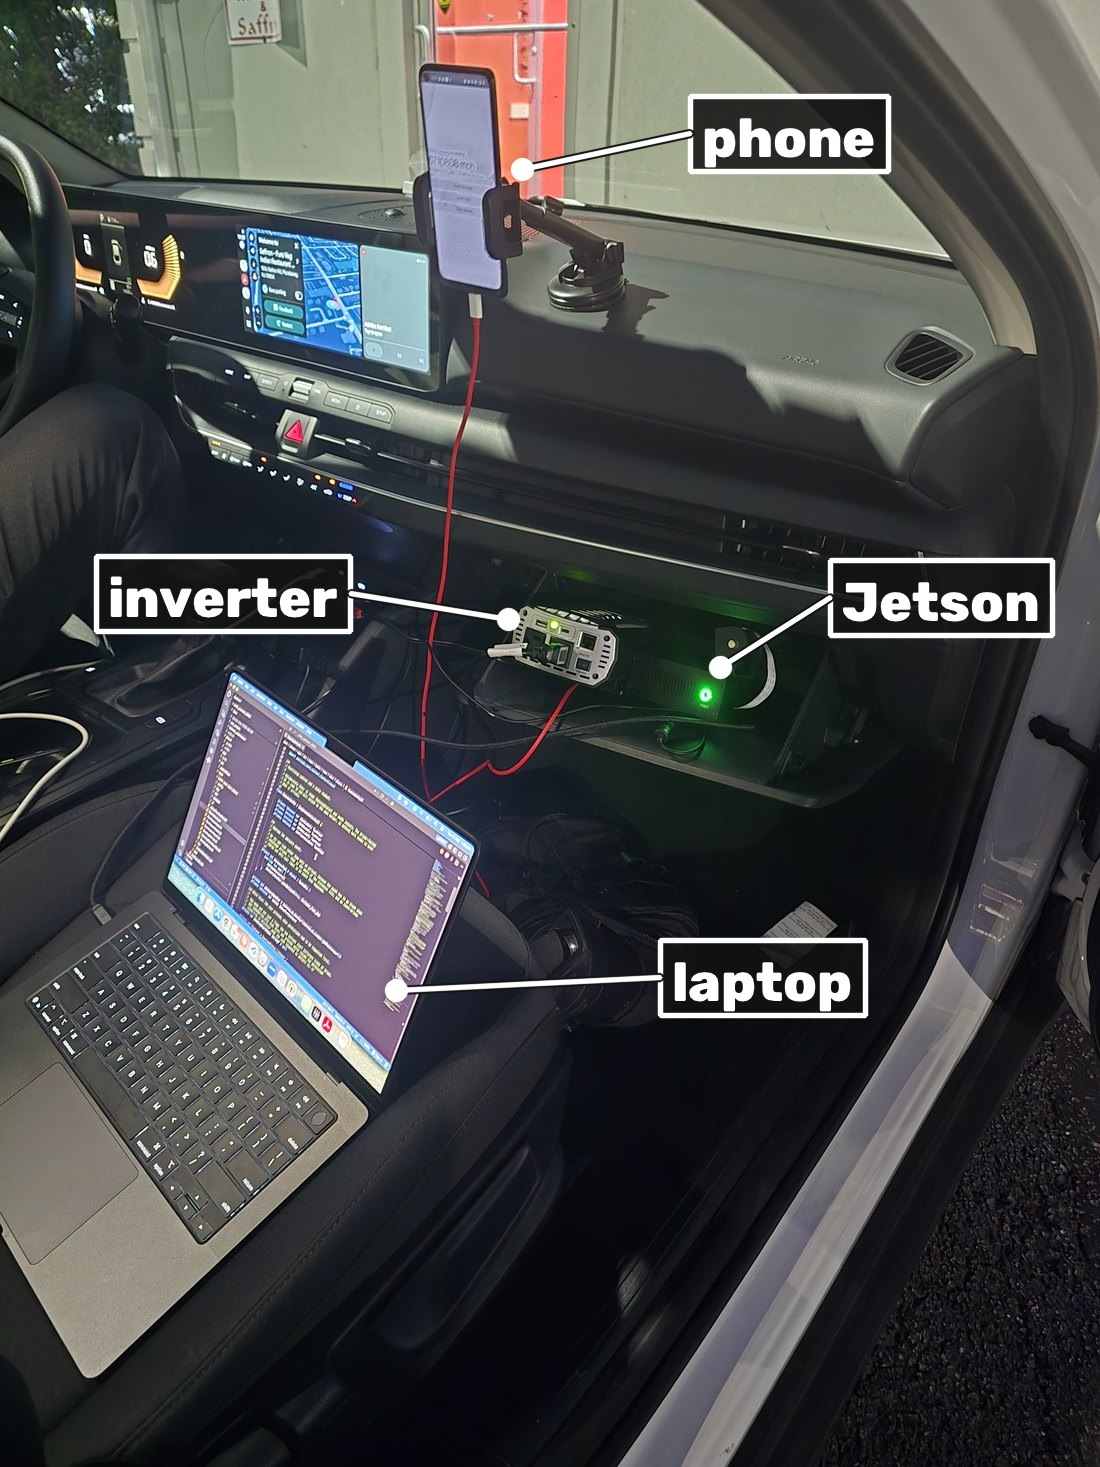
\includegraphics[width=0.72\linewidth]{images/rig_dashboard.jpg}\\[2pt]
{\footnotesize (a) Everything added to the vehicle.}\\[4pt]
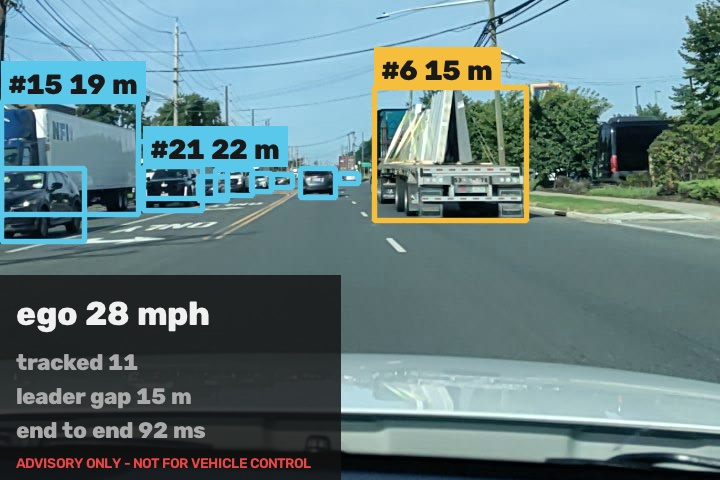
\includegraphics[width=\linewidth]{images/perception_drive_frame.jpg}\\[2pt]
{\footnotesize (b) What it computes, on a recorded drive frame.}
\caption{The deployment prototype. The phone supplies the camera, GPS and inertial unit and carries the display; the Jetson runs perception, the policy and the safety gate; the inverter is the only connection to the car. The laptop is for debugging and is not part of the rig. Nothing reaches the throttle, the brakes, the steering or the vehicle bus. In (b), we show the camera perception module. The leader in the ego lane is amber and the other tracked vehicles are cyan.}
\label{fig:teaser}
\end{figure}


A free-flow road network can jam without any apparant cause, without a crash or a fixed bottleneck. A small burst of inflow traffic can push the local density past a critical value and the queue then feeds itself until the demand drains away~\cite{bhardwaj2023understanding,sugiyama2008traffic}. This phenomenon in the literature is coined as a sudden traffic jam. Several prior studies have focussed on mitigating such traffic flow instabilities. For example, learned controllers that smooth mixed-autonomy traffic report gains at low penetration in microscopic simulators~\cite{wu2017flow,vinitsky2018benchmarks,kreidieh2018dissipating}.

Another work in this space introduced the concept of self-regulating cars~\cite{self_regulating_cars}. \cite{bhardwaj2023understanding} notes that the fundamental diagram of traffic flow provides an explanation for the underlying process of sudden traffic jams. The flow rises with density to a critical point and falls after it~\cite{greenshields1935study,lighthill1955kinematic,richards1956shock}. Therefore, a controller that holds density below that point protects throughput, and it does not need to know anything about the rest of the network to do so.

Earlier work introducing self-regulating cars built such a controller and measured it. That work divided the Mainz highway network into twelve super-segments, learned a policy that assigns each super-segment a desired speed, and applied that speed to the vehicles on it. In PTV Vissim the policy raised throughput by 5\% and cut average delay by 13\% against no control. The result holds at partial adoption and improves as the controlled fraction grows. Its orchestration model is centralized. A central coordinator collects the network state, computes the action, and sends every participating vehicle its desired speed.

While the results shown by \cite{self_regulating_cars} and others are promising, they remain limited to simulations. Deployment, an extremely important and difficult step for impact, is generally treated as an engineering detail rather than as a research question. What it would cost goes unreported, except for a few exceptions~\cite{stern2018dissipation,lee2024traffic}.

This paper tackles deploying self-regulating cars as its central question. Ease of adoption is decided by the size of the change, because the controller's benefit grows with the fraction of vehicles carrying it. That fraction is therefore the quantity a deployment design has to maximise, and anything raising the cost of one installation lowers it. Judged this way, two properties of the centralized model are expensive. The first is the observation: the policy reads six features per super-segment, and four of them are vehicle-level ground truth a vehicle cannot easily obtain. The second is the cloud coordinator, which has to be built, paid for, kept available and trusted, and which sits inside the control loop. Other designs put a floor under the same cost elsewhere, whether through a purpose-built vehicle~\cite{lee2024traffic}, a roadside sensor~\cite{arnold1998ramp,papageorgiou2002freeway} or a per-vehicle service contract~\cite{self_regulating_cars}. The target here is the opposite: the least that has to be added to a vehicle that already exists. We call this the minimum viable deployment and discuss it in Section~\ref{sec:vision}. Our proposed solution is summarized in Table~\ref{tab:bom}. The computer is an NVIDIA Jetson Orin Nano developer kit, listing at about US\$250~\cite{nvidia2025orinnano}, and the phone used for the drives reported here is a OnePlus Nord N10 (2021 model), a mid-range handset rather than a flagship. Figure~\ref{fig:teaser} is the prototype we built, installed and running.

\begin{table}[t]
\centering
\caption{What a vehicle has to acquire. No part of this system is installed on the road, and no part of it is wired into the vehicle.}
\label{tab:bom}
\small
\begin{tabular}{p{0.28\linewidth}p{0.35\linewidth}p{0.18\linewidth}}
\toprule
\textbf{Part} & \textbf{Supplies} & \textbf{Cost} \\
\midrule
Jetson Orin Nano developer kit & perception, policy, safety gate & US\$250 \\
Android phone & camera, GPS, inertial unit, display, cellular & US\$150 \\
Mount, 12\,V inverter, cable & power and mounting & US\$100 \\
\bottomrule
\end{tabular}
\end{table}

The division of labour inside the rig is as follows: the phone captures and forwards, the Jetson interprets and decides. Nothing is wired to the throttle, the brakes, the steering or the vehicle bus. The only connection to the vehicle is a 12\,V power lead, so the installation changes no system the vehicle already depends on. The advisory is shown to the driver using the phone display, and they decide their level of compliance. That is an arrangement a navigation application already runs. Mobile telematics platforms operate the same driver-facing rail at the scale of tens of millions of drivers~\cite{cmt2025,samsara2025}. This human-in-the-loop design supports our claim about deployability, namely that the interface needs no new hardware, no new habit, and no regulatory change.

\noindent\textbf{Scope of the work.} No advisory this project computed has ever been acted on. On every drive, the human drove without interfere while the Jetson rendered a recommended speed on the phone's display. There are two independent reasons for this. An experiment in which an advisory influences a human driver requires approval from an institutional review board, which this project does not hold. One instrumented vehicle also cannot produce a flow effect, so a compliance experiment on a single car would establish nothing about throughput or delay. In this paper ``deployed'' means that the system ran on a road and computed its outputs there. It does not mean that the recommendations were acted on. The flow-level claim is made in simulation for the same reason.

\noindent\textbf{Contributions.}
\begin{itemize}[leftmargin=1.2em,itemsep=1pt,topsep=2pt]
\item A vehicle-side realization of the self-regulating-cars deployed using commodity parts, with a sensing scheduler that sets every sensor's sampling rate at run time (Sections~\ref{sec:vision} and~\ref{sec:architecture}).
\item A measured account of running the system on a road: eight drives, 152.8 minutes on vehicle power, with per-stage timing and field provenance, and the deployment experiences that were produced. The phone overheated from its own load and from sunlight on the windscreen, and a ninety-degree camera rotation sent detection to zero (Section~\ref{sec:eval}).
\item A flow-level measurement of the observation change. On a SUMO port of the same Mainz network, a policy restricted to the five fields a traffic API returns gains $230 \pm 44$\,veh/h over no control, and the original six-feature policy gains $224 \pm 61$\,veh/h (Section~\ref{sec:simulation}).
\end{itemize}
